\chapter{Evaluation问题}

首先我们来整理一下现在所有的前提假设,首先我们有所有可能的状态变量$i_t$的状态集合$Q$和所有可能的状态变量$o_t$的观测集合$V$:

\begin{equation}
    Q=\{q_1,q_2,\cdots,q_N\}, \ \ \ \ V=\{v_1,v_2,\cdots,v_M\},
\end{equation}

其中$N$是可能的状态数,$M$是可能的观测数。

$I$是长度为$T$的状态序列,$O$是对应的观测序列:
\begin{equation}
    I=(I_1,I_2,\cdots,I_T),\ \ \ \ O=(O_1,O_2,\cdots,O_T)
\end{equation}

同时我们有参数$\lambda=(\pi,\mathcal{A},\mathcal{B})$,其中$\pi$为初始状态概率向量
\begin{equation}
    \pi = (\pi_i)_{N},\ \ \ \ \pi_i=P(I_1=q_i),\ i=1,2,\cdots,N
\end{equation}

$\mathcal{A}$是\textsl{状态转移矩阵},
\begin{equation}
    \mathcal{A}=[a_{ij}]_{N\times N}
\end{equation}

其中$a_{ij}=P(I_{t+1}=q_j|I_t=q_i)$。

$\mathcal{B}$是\textsl{观测概率矩阵},
\begin{equation}
    \mathcal{B}=[b_j(k)]_{N\times M}
\end{equation}

其中$b_{j}(k)=P(O_{t}=v_k|I_t=q_j)$。



\section{直接计算}

直接计算就是直接依照概率图模型直接展开,但是计算量很大,计算复杂度是$O(TN^T)$阶的。
\begin{equation}
    P(O|\lambda)=\sum_{I_1}\cdot\sum_{I_2}\cdot\cdots\cdot \sum_{I_T}\pi_{i_1}\prod_{t=2}^{T}a_{i_t-1,i_t}\prod_{t=2}^{T}b_{i_t}(O_t)
\end{equation}

一共有$T$个状态,每个状态$N$种可能,所以复杂度为$\mathcal{O}(N^T)$

\section{前向算法}


首先我们先展示一下Hidden Markov Model的拓扑结构
\begin{figure}[H]
    \centering
    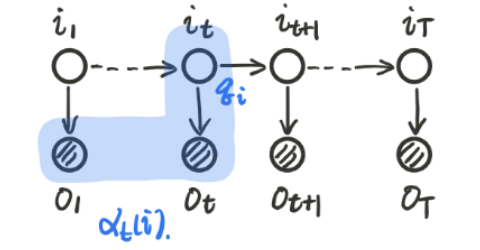
\includegraphics[scale=0.5]{figures/前向算法的拓扑结构.png}
    \caption{前向传播算法的拓扑结构}
\end{figure}

前向算法的主要思想是,在之前所有的观测变量$O_t$的前提下求出当前时刻的隐变量的概率,即
\begin{equation}
    P(O|\lambda)=\sum_{i=1}^{n} P(O,I_T=q_i|\lambda)=\sum_{i=1}^{n} \alpha_T(i)
\end{equation}

我们希望的是从$\alpha_1(i)$开始,一步一步向前推从而获得$\alpha_T$,也就是我们需要的是$\alpha_t(i)$和$\alpha_{t+1}(i)$具有某种递推关系,
下面我们来推导这种关系

\begin{mdframed}
    \begin{proposition}
        $\alpha_{t+1}(j)=b_j(O_{t+1})\cdot a_{ij}\cdot\alpha_i(i)$,其中$b_j(O_{t+1})=\sum_{k=1}^{M}\nu_k$
    \end{proposition}
\end{mdframed}

\begin{mdframed}[linewidth=0pt,backgroundcolor=gray!10]

    \begin{equation}
        \begin{aligned}
            \alpha_{t+1}(j)&=P(O_1,\cdots,O_t,O_{t+1},I_{t+1}=q_j|\lambda)\\
            &=\sum\limits_{i=1}^{N}P(O_1,\cdots,O_t,O_{t+1},I_{t}=q_i,I_{t+1}=q_j|\lambda)\\
            &=\sum\limits_{i=1}^{N}\underbrace{P(O_{t+1}|I_{t+1}=q_j,\lambda)}_{A}\underbrace{P(O_{1},O_{2},\cdots,O_{t},I_t=q_i,I_{t+1}=q_j|\lambda)}_{B}
        \end{aligned}
    \end{equation}

    其中$A$式刚好是观测概率矩阵的元素$b_j(O_{t+1})$

    \begin{equation}
        A=P(O_{t+1}|I_{t+1}=q_j,\lambda)=\sum_{k=1}^{M}b(O_{t+1}=\nu_k|I_{t+1=q_j},\lambda)=b_j(O_{t+1})
    \end{equation}

    主要来关注$B$,我们发现$B$还有关于$t+1$的项,我们想要这一项只和$t$及其之前的序列相关,因此对$B$做继续展开
    \begin{equation}
        \begin{aligned}
            B&=P(O_{1},O_{2},\cdots,O_{t},I_t=q_i,I_{t+1}=q_j|\lambda)\\
            &=P(I_{t+1}=q_j|O_{1},O_{2},\cdots,O_{t},I_t=q_i,\lambda)\cdot P(O_{1},O_{2},\cdots,O_{t},I_t=q_i|\lambda)\\
        \end{aligned}
    \end{equation}

    根据齐次马尔可夫假设
    \begin{equation}
        B=P(I_{t+1}=q_j|I_t=q_i,\lambda)\cdot P(O_{1},O_{2},\cdots,O_{t},I_t=q_i|\lambda)\\
    \end{equation}

    上式子左边第一项刚好是转移矩阵,第二项刚好是$\alpha_t(i)$所以
    \begin{equation}
        B=a_{ij}\cdot \alpha_t(i)
    \end{equation}

    然后我们把$A$和$B$最后的计算结果带回$\alpha_{t+1}(j)$
        \begin{equation}
            \alpha_{t+1}(j)=b_j(O_{t+1})\cdot a_{ij}\cdot \alpha_t(i)
        \end{equation}

\end{mdframed}

这个递推关系有什么意义呢?我们的联合概率分布是
\begin{equation}
    P(O|\lambda)=\sum_{i=1}^{n} P(O,I_T=q_i|\lambda)=\sum_{i=1}^{n} \alpha_T(i)
\end{equation}

利用递推关系,我们可以从简单的$\alpha_1$开始,用$\alpha_1$推导$\alpha_2$、$\alpha_2$推导$\alpha_3\cdots$,以此类推,最终算出来$\alpha_T(j)$,代入求和式就是联合概率分布。
而$\alpha_1$是只和一个状态结点和一个观测结点相关,因此是容易确定的。
\begin{figure}[H]
    \centering
    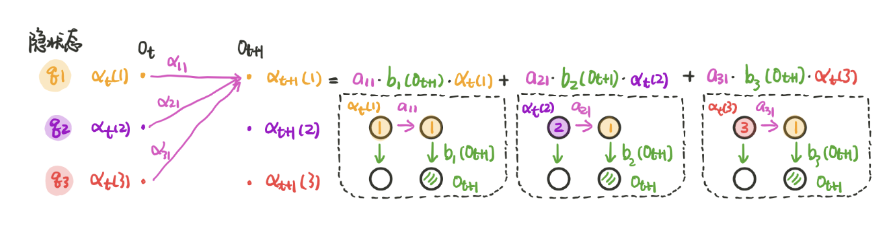
\includegraphics[scale=0.5]{figures/HMM前向传播示意图.png}
    \caption{HMM前向传播示意图}
\end{figure}

前向算法实际上是基于“状态序列的路径结构”递推计算联合概率分布的算法。其关键在于\textsl{局部计算前向概率,利用路径结构将前向概率递推到全局,从而减少每一次计算直接引用前一个时刻的计算结果,避免重复计算},
每次计算,隐状态的状态空间数为$N$,序列长度为$T$,因此这样利用前向计算算法的计算量是$O(N^2T)$阶的。


\section{后向算法}

后向概率的推导实际上比前向概率的理解要难一些,前向算法实际上是一个联合概率,而后向算法则是一个条件概率,所以后向的概率实际上比前向难求很多。

\begin{figure}[H]
    \centering
    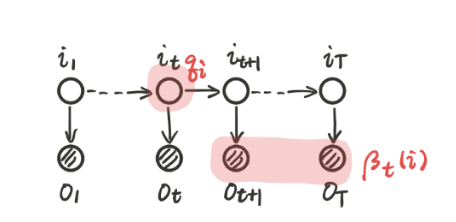
\includegraphics[scale=0.5]{figures/后向算法示意图2.png}
    \caption{后向算法示意图}
\end{figure}

我们设$\beta_{t}(i)=P(O_{t+1},\cdots,O_{T}|I_t=q_i,\lambda)$,计算观测的联合概率分布
\begin{equation}
    \begin{aligned}
        P(O|\lambda)&=P(O_1,O_2,\cdots,O_N|\lambda)\\
        &=\sum_{i=1}^{N}P(O_1,O_2,\cdots,O_N,I_1=q_i|\lambda)\\
        &=\sum_{i=1}^{N}P(O_1,O_2,\cdots,O_N|I_1=q_i,\lambda)\cdot P(I_1=q_i|\lambda)\\
        &=\sum_{i=1}^{N}P(O_1|O_2,\cdots,O_N,I_1=q_i|\lambda)\cdot P(O_2,\cdots,O_N,I_1=q_i|\lambda)\cdot\pi_i\\
        &=\sum_{i=1}^{N}P(O_1|I_1=q_i,\lambda)\cdot \beta_i(i)\cdot \pi_i\\
        &=\sum_{i=1}^{N}b_i(O_1)\cdot \beta_1(i)\cdot \pi_i
    \end{aligned}
\end{equation}

现在我们成功找到了$P(O|\lambda)$和第一个状态之间的关系,如下图所示
\begin{figure}[H]
    \centering
    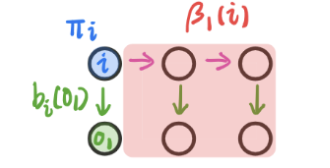
\includegraphics[scale=0.5]{figures/与第一个状态的关系.png}
    \caption{$P(O|\lambda)$与第一个状态的关系}
\end{figure}

现在我们要通过递推找最后一个状态和第一个状态的关系
\begin{equation}
    \begin{aligned}
        \beta_t(i)&=P(O_{t+1},\cdots,O_{T}|I_t=q_i)\\
        &=\sum_{j=1}^{N}P(O_{t+1},\cdots,O_{T}|I_t=q_i,i_{t+1}=q_j)\cdot P(I_{t+1}=q_j|I_t=q_i)
    \end{aligned}
\end{equation}

根据概率图模型,$I_t$和$t+1$后面所有的状态都没有关系,因此
\begin{equation}
    \begin{aligned}
        \beta_t(i)&=\sum_{j=1}^{N}P(O_{t+1},\cdots,O_T|I_{t+1}=q_j)\cdot a_{ij}\\
        &=\sum_{j=1}^{N}P(O_{t+1}|O_{t+1},\cdots,O_T,I_{t+1}=q_j)\cdot \underbrace{P(O_{t+2},\cdots,O_T|I_{t+1}=q_j)}_{\beta_{t+1}(j)}\cdot a_{ij}\\
        &=\sum_{j=1}^{N} b_j(O_{t+1})\cdot \beta_{t+1}(j)\cdot a_{ij}
     \end{aligned}
\end{equation}

马尔可夫链中每一个状态都是后一个状态的充分统计量,与之前的状态没有关系
\begin{equation}
    P(O_{t+1},\cdots,O_T|I_{t+1}=q_j,I_t=q_i)=P(O_{t+1},\cdots,O_T|I_{t+1}=q_j)
\end{equation}

通过这样的迭代方法从后往前推就可以得到$\beta_1(i)$的概率了,从而推断$P(O|\lambda)$。

\begin{figure}[H]
    \centering
    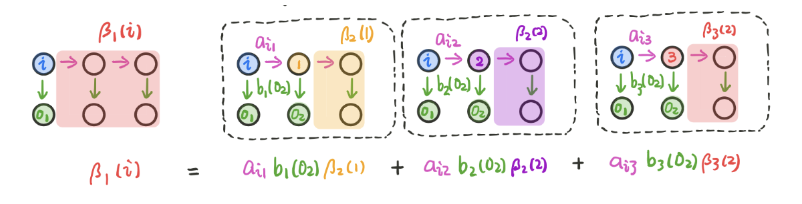
\includegraphics[scale=0.5]{figures/后向算法示意图.png}
    \caption{后向传播算法的拓扑结构}
\end{figure}